\cotefile{156-6}
\scanpage{81}
\mspage{80}
\uline{At} 11 bis \quad Soit $F$ une figure, $(F'_i)_{i\in I}$ une famille filtrante croissante de raffinements de $\unsure{F|\mathbf{F}}$. Supposons que pour tout $X\in\widetilde F$, la famille des $F'_i\mid X$ \deleted{\unsure{soit stationnaire}}. \inserted{\unsure{admette} un $\operatorname{Sup}$ (soit $F_X$)}. Alors $F'=\operatorname{Sup} F'_i$ existe

NB \quad \unsure{Ça|Sa} résulte aussitôt de \uline{$\unsure{\mathrm{At}^{+}|\mathrm{At}}$} 11, et \unsure{ça|se} implique At 11 moyennant \uline{At} $11'$ (critère de compatibilité) \deleted{Mais \unsure{Ce|Ça|c'}} \unsure{Son|Sa} \unsure{caractère|variation} sympathique, c'est d'isoler le caractère ``condition de locale finitude''

Ainsi, on songe à s'arrêter aux axiomes ``réduits à l'os''
\[
\mathrm{At}\,9_{\Sigma},\quad \mathrm{At}\,10,\quad \mathrm{At}\,11\ \text{bis}
\]
\margin{ici At 12 a disparu}
\margin{$\nearrow$ n'a rien à voir avec les lieux, et devrait se formuler avant les axiomes sur les lieux (\deleted{\unsure{critère}} d'existence des $\sup$ \unsure{filtrantes|filtrants})}
\unsure{le|Le} seul petit ennui étant dans la formulation de $\mathrm{At}\,9_{\Sigma}$, un peu \unsure{abracadabrante}, à cause du choix d'un $\Sigma$. Si on veut éviter $\mathrm{At}\,9_{\Sigma}$, on est réduit à nouveau à
\[
\mathrm{At}\,9,\quad \deleted{\mathrm{At}\,10,},\quad \mathrm{At}\,11\ \text{bis},\ \mathrm{At}\,12
\]
\margin{ici At 10 a disparu}
et on perd seulement un critère de compatibilité universel par lieux, $\mathrm{At}\,9_{\Sigma}$, bien sympathique.
% slanted
\margin{dans les deux \unsure{syst.} d'axiomes At 11 et At $11'$ ont disparu, au profit de At 11 bis qui est dans les deux}

\unsure{Il|Je} \unsure{faudra|faudrai} le \unsure{récupérer} quand on passera à la saturation de l'\unsure{atelier|atlas}, \deleted{\unsure{pour|pour que}} en n'oubliant pas, dans la définition d'un \unsure{atelier|atlas} saturé, d'inclure $\mathrm{At}\,9'=\mathrm{At}\,9_{\Sigma}$ (pour $\Sigma={}$tous les \unsure{ens.|m.} ordonnés).
\scanpage{82}
\mspage{81}
\figure{\begin{tikzpicture}\draw[line width=.4pt] (0,0) -- (1.5,0);\end{tikzpicture}}

J'en viens aux \deleted{axiomes} \uline{subdivisions}, dont il n'avait pas encore été question jusqu'à présent ! J'ai envie de poser

\deleted{\uline{At 13}} \inserted{Proposition} \quad Soient $F$ une figure, $F'\ll F$. Supposons qu'il existe une figure $G$ non vide, avec $G\parallel F'$, $G\mathrel{\overline{\parallel}}F$. Alors il existe $\unsure{\bar{\text{m}}|=}$ une telle figure avec $G\ll F$.

\deleted{En vertu de} On pourra alors prendre pour $G$ \unsure{une|un} $X\in\unsure{M|\mathcal M}$, et $\bar{\text{m}}$ un $x\in\unsure{L|\mathcal L}$, \deleted{\unsure{pour}} en prenant n'importe quel $X$ \unsure{dans|en} $\operatorname{Omb}(\unsure{G|X})$ resp. \deleted{\unsure{dans}} $x$ dans $\operatorname{Omb}(G)$.

(NB on se rappellera de \unsure{(1.58.|C1.58.|Cl.58.} page 59)

Pour trouver \unsure{une|un} énoncé minimal qui implique la prop, notons que dans la donnée initiale, $\deleted{\unsure{d|F}}G$, l'hypothèse $G\mathrel{\overline{\parallel}}F$ signifie aussi (par At 9) qu'il existe $\deleted{\unsure{x}}y\in\unsure{\operatorname{Om}|\operatorname{om}}G$, \inserted{$x\in\operatorname{om}(F)$,} tels que $\deleted{\unsure{x\mathrel{\overline{\parallel}}F|x\mathrel{\overline{\parallel}}y}}$ $x\deleted{\unsure{\in|o}}\mathrel{\overline{\parallel}}y$, \inserted{et on aura \unsure{pourtant} $y\parallel\deleted{G}F'$!} Soit alors $X\in\widetilde F$ tel que $x\in\operatorname{om}(X)^{\circ}$ i.e. $x\ll X$.
\diagram{\begin{tikzcd}[ampersand replacement=\&,row sep=1pt,column sep=5pt]
F' \& \ll \& F \& {}\\
\unsure{\rotatebox{90}{$\leqslant$}|\rotatebox{90}{$\leq$}} \& \& \rotatebox{90}{$\leqslant$} \& {}\\
F'_X \& \ll \& X \& {}\\
{} \& \& \rotatebox{90}{$\ll$}\,{\scriptstyle\circ} \& {}\\
{} \& \& x \& y
\end{tikzcd}}
\scanpage{83}
\mspage{82}
On veut remplacer la situation initiale par
\diagram{\begin{tikzcd}[ampersand replacement=\&,row sep=0pt,column sep=6pt]
F'_X \& \ll \& X \& y \& \qquad \text{(i.e. \unsure{cas|en} }F\in\unsure{M|\mathcal M},\\
{} \& {} \& \deleted{\unsure{\rotatebox{90}{$\ll$}}} \& {} \& G\in\unsure{L|\mathcal L}\text{)}\\
{} \& {} \& \deleted{\unsure{x}} \& {} \& {}
\end{tikzcd}}
en utilisant \deleted{\unsure{deux|de}} \unsure{de} plus l'existence d'un $x\in\unsure{\operatorname{omb}|\operatorname{Omb}}(X)^\circ$ tel que $x\mathrel{\overline{\parallel}}y$. Supposons qu'on puisse trouver $\deleted{y}z\in\operatorname{omb}(X)$ \unsure{telles|tels} que $\deleted{y}z\parallel F'_X$. On aura $\deleted{\unsure{y}}z\ll X\leq F$ donc $\deleted{y}z\ll F$, prouvons que $\deleted{y}z\parallel\deleted{\unsure{G}}F'$ (donc on gagne, en prenant $G=\deleted{y}z'$).

\deleted{Mais en effet, \deleted{\unsure{on verra par $y'$|on verra pour $y'$} \unsure{$\ll$}} \inserted{par At 9 il suffit de} vérifier que $\forall\,\deleted{\unsure{x}}z'\in L,\ \deleted{\unsure{x}}z'\ll F'$, on ait $z'\parallel z$. Si $z'\ll F'_X$, cela résulte de $F'_X\parallel z$. Sinon, \unsure{$\perp$|il}.} Cela va résulter du

\uline{Lemme} \quad \deleted{\unsure{Soit}}\unsure{Soient}
\diagram{\begin{tikzcd}[ampersand replacement=\&,row sep=1pt,column sep=5pt]
F' \& \ll \& F\\
\unsure{\rotatebox{90}{$\leqslant$}|\rotatebox{90}{$\leq$}} \& {} \& \rotatebox{90}{$\leqslant$}\\
F'_G \& \ll \& G\\
{} \& {} \& \rotatebox{90}{$\ll$}\\
{} \& {} \& H
\end{tikzcd}}
Pour que \deleted{$H$ soit \unsure{di}} l'on ait $H\parallel F'$, il (f et)s que $H\parallel F'_G$.

(On l'appliquera à $G=X$, $H=z$) Supposons en effet $H\parallel F'_G$, prouvons $H\parallel F'$, donc que \deleted{\unsure{prouvons}}
\[
x'\in\operatorname{omb} F',\ \unsure{y|x}\in\operatorname{omb} H\ \Longrightarrow\ x\parallel \unsure{y'|x'}.
\]
\margin{\rule[-1.5ex]{.4pt}{5ex}\,NB \unsure{OPS|OBS|OFS} $H=\deleted{\unsure{G}}y$ $F'=x'$}
On le sait par hyp. si $x\in\operatorname{omb} F'_G=\operatorname{omb} F'\cap\operatorname{omb} G$. Si $x\in\operatorname{omb} F'\setminus\operatorname{omb} F'_G$
\scanpage{84}
\mspage{83}
Considérons
\diagram{\begin{tikzcd}[ampersand replacement=\&,row sep=1pt,column sep=5pt]
x' \& \ll \& F' \& \ll \& F\\
\unsure{\rotatebox{90}{$\leqslant$}|\rotatebox{90}{$\leq$}} \& {} \& \rotatebox{90}{$\leqslant$} \& {} \& \rotatebox{90}{$\leqslant$}\\
x'_G \& \ll \& F'_G \& \ll \& G\\
{} \& {} \& {} \& {} \& \rotatebox{90}{$\ll$}\\
{} \& {} \& {} \& {} \& x
\end{tikzcd}}
Comme $x'_G\leq x'$, et $x'\in\unsure{L|\mathcal L}$, on aura $x'_G=x'$ ou $x'_G=\emptyset$, et comme $x'\not\ll F'_G$ par hyp. on a $x'_G=\emptyset$. Mais cela signifie aussi que $\deleted{\unsure{\operatorname{omb}(\,)|\operatorname{omb}(/}}x'\in\operatorname{omb}(F)\setminus\operatorname{omb}(G)$, donc $x$ et $x'$ appartiennent à des strates \unsure{ouvertes} différentes de $\operatorname{omb}(F)$, donc $x\parallel x'$ par At 10.

Nous allons donc poser

\uline{At 13} \quad Soi\deleted{\unsure{ent|en}}\unsure{t|ent} $F\ll X$, avec $X\in\unsure{M|\mathcal M}$.
% slanted
\margin{\uline{NB} At 8, At 9, $9_{\Sigma}$, At 13 sont des axiomes d'existence de ``beaucoup'' de lieux.}
% slanted
\margin{``Axiome \unsure{du support|des supports}'' (dans \unsure{le critère|la nature} d'existence de suffisamment de lieux).}
% slanted
\margin{Avec la notion de support abstrait associé à $(\unsure{\mathcal F|\mathscr F},\leq)$ ou à $(M,\leq)$, l'hypothèse signifie aussi que $\operatorname{supp} F\unsure{\not\subseteq|\neq}\deleted{\unsure{\emptyset}}\operatorname{supp}G$, et At 13 dit que \unsure{il|ça} \deleted{\unsure{se|ça}} \unsure{si|se} \unsure{peut|pour} tester déjà ça avec les lieux}
\deleted{\unsure{On}} Supposons qu'il existe $G\in\mathcal F$, $G\neq\emptyset$, $G\parallel F$, $G\mathrel{\overline{\parallel}}X$ (NB on \deleted{\unsure{pourra}} sait déjà qu'on pourra alors prendre $G\in L$). Alors il existe $x\in\operatorname{omb} X$, tel que $\deleted{F\parallel x}\ x\parallel F$ (et bien sûr on aura alors $x\mathrel{\overline{\parallel}}X$).

\uline{Corollaire 1} \quad Soit $F'\ll F$. Conditions équivalentes :
\begingroup\csname tagsleft@true\endcsname
\[
\forall G\in\mathcal F,\quad G\parallel F'\ \Longrightarrow\ G\parallel F
\tag*{(i)}
\]
\inserted{(donc $G\parallel F'\Longleftrightarrow G\parallel F$)}
\[
\deleted{\unsure{\exists x|\exists}} \ \text{Pour tout }x\unsure{{,}|{.}}\in\unsure{\operatorname{domb}|\operatorname{omb}}(X),\ \text{on a }x\mathrel{\overline{\parallel}}F'
\tag*{(ii)}
\]
\endgroup
\scanpage{85}
\mspage{84}
(iii) \deleted{Il n'existe pas de} \inserted{Pour \unsure{toute|tout} $\overline{F'}$}, avec
\[
F'\leqslant\overline{F'}\ll F
\]
on a $F'=\overline{F'}$, i.e $F'$ est maximal parmi les raffinements de $F$, ordonnés par $\leqslant$

\deleted{(iv) Pour tout $F'$ avec}
\[
\deleted{F'\ll\overline{F'}\ll F}
\]
\deleted{on a $F'=\overline{F'}$, i.e. $F'$ est maximal parmi les raffinements de $F$, ordonnés par $\ll$.}

\uline{Dém} \quad $\mathrm{(i)}\Longleftrightarrow\mathrm{(ii)}$ n'est autre que la prop. (\unsure{validée} par At 13), compte tenu de la remarque qui la suit.

\deleted{$\unsure{\mathrm{(ii)}|\mathrm{(iii)}}\Longrightarrow\mathrm{(iii)}$ est évident}

$\mathrm{(iii)}\Longrightarrow\mathrm{(ii)}$ \deleted{Car si \deleted{\unsure{on}} (ii) n'était \unsure{vraie|véri}} \inserted{i.e. $\overline{\mathrm{(ii)}}\Longrightarrow\overline{\mathrm{(iii)}}$.} En effet si $\deleted{\unsure{\exists x\in}}$ on a $x\in\operatorname{omb} F$, avec $\unsure{a|x}\parallel F$, cons\deleted{\unsure{é|i}}\unsure{idérons}
\[
F'\vee x=\overline{F'}
\]
prouvons que l'on a $\overline{F'}\ll F$ (ce qui montrera $\overline{\mathrm{(iii)}}$, car $F'\unsure{\lneq|\not\leqslant|\neq}\overline{F'}$). Or \deleted{\unsure{il suffit|il convient} donc de prouver cela} par At 4 cela se prouve strate par strate, on gagne.

\deleted{\uline{Prop} \unsure{Soient|Soit} $F$ figure,}

Il reste à prouver que $\mathrm{(ii)}\Longrightarrow\unsure{\mathrm{(iv)}|\mathrm{(iii)}}$. \deleted{Prouvons d'abord $\mathrm{(ii)}\Longrightarrow\mathrm{(iii)}$.} Si dans (iii), on avait $F'\neq\overline{F'}$, soit $\deleted{\unsure{x}}X\in\widetilde{\overline{F'}}\setminus\widetilde{F'}$, $x\in\operatorname{omb}(X)\unsure{\}|y}$ alors $x\ll\overline{F'}\ll F$ donc $x\ll F$, et $x\parallel F'$, \unsure{contrairemt|contrairement} à (ii). \deleted{Ainsi (i)(ii)(iii) sont \unsure{équivalents|équivalentes} et impliqués par (iv).} Mais impliquent ils (iv) ?
\scanpage{86}
\mspage{85}
% slanted
\margin{\uline{NB} \unsure{Si on ne|Sans} \unsure{suppose|supposer} At 13, on définira néanmoins $F'\unsure{\preccurlyeq|\preceq}F$ par $\deleted{\unsure{G|E}}F'\ll F+$ condition de supports \ldots}
\uline{Définition} \quad Quand ces conditions sont satisfaites, on dit que $F'$ est une \uline{subdivision} de $F$, ou $F$ une \uline{surdivision} (ou un \uline{regroupement}) de $F'$, et on ecrit
\[
F'\preccurlyeq F\ .
\]
% slanted
\margin{\uline{NB} Ça implique $\widetilde{F'}\unsure{\mathbin{-}|\to}\widetilde F$ \uline{surjectif} (à \unsure{expliciter} en prop.)}

\uline{Proposition} \quad La relation $F'\preccurlyeq F$ dans $\unsure{\mathcal F|\mathscr F}$ est une relation d'ordre

Elle est évidemment reflexive. Prouvons
\[
F''\preccurlyeq F'\preccurlyeq F\ \Longrightarrow\ F''\preccurlyeq F
\]
% slanted
\margin{Plus \unsure{généralt|généralemt} si $F''\ll F'\ll \unsure{F|F'}$ d'où $F''\ll F$, et si deux parmi ces $\ll$ sont $\preccurlyeq$, le troisième aussi.}
Soit $G\in\mathcal F$, supposons $G\parallel F''$, prouvons $G\parallel F$. En effet, on a $G\parallel F'$ car $F''\preccurlyeq F'$, donc $G\parallel F$ car $F'\preccurlyeq F$, OK.
% slanted
\margin{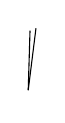
\begin{tikzpicture}[baseline=-.4ex,x=1ex,y=1ex]\draw (0,0) -- (.15,5);\draw (0,0) -- (.65,5.2);\end{tikzpicture}\,\uline{Mieux} Si $F''\ll F'\ll F\unsure{\in|\epsilon}$, \unsure{alors} $(F''\preccurlyeq F)\deleted{\unsure{\text{éq}|\Longrightarrow}}\Longleftrightarrow(F''\preccurlyeq F'\text{ et }F'\preccurlyeq F)$}

\uline{Proposition} \quad Considérons
\diagram{\begin{tikzcd}[ampersand replacement=\&,row sep=2pt,column sep=5pt]
F' \& \ll \& \deleted{\unsure{G}}F\\
\unsure{\rotatebox{90}{$\leqslant$}|\rotatebox{90}{$\leq$}} \& {} \& \rotatebox{90}{$\leqslant$}\\
\deleted{\unsure{G|E}}F'_G \& \ll \& G
\end{tikzcd}}
Si $F'\preccurlyeq F$, alors $F'_G\preccurlyeq G$.

En effet, \deleted{soit $K\in\mathcal F$, avec $x$} \inserted{il suffit de voir que \deleted{\unsure{l'il|l'on}}} $\deleted{\forall x\in\unsure{\operatorname{om}|\operatorname{omb}}}$ pour $x\in\operatorname{omb}(G)$, on a $x\mathrel{\overline{\parallel}}F'_G$. Mais si on avait $x\parallel F'_G$, on aurait $x\parallel F'$ par le lemme p.~\unsure{87|82}, \unsure{contrairemt|contrairement} à $F'\preccurlyeq F$, qed.

\uline{Corollaire 1} \quad Soit $F'\ll F$, et $F_i\leqslant F$ $(i\in I)$ tels que $\operatorname{Sup} F_i=F$. Soit $F'_i=F'\mid F_i$ le raffinement de $F_i$ induit. Alors $F'\preccurlyeq F$
\[
\text{\unsure{ssi}}\quad F'_i\preccurlyeq F_i\qquad\forall i\in I.
\]
\scanpage{87}
\mspage{86}
Nécessité résulte de la prop. Pour la suffisance, soit $x\in\operatorname{omb}\deleted{\unsure{G|E}}F$, prouvons qu'on ne peut avoir $x\parallel F'$. Comme $\deleted{\unsure{\operatorname{om}}}\operatorname{omb}F=\bigcup_i\operatorname{omb}(F_i)$, $\deleted{\unsure{\text{on}|{-}}}\exists i\deleted{\unsure{\text{a}|{-}}}$ t.q. $x\in\operatorname{omb}F_i$. Mais alors, comme $F'_i\unsure{\preccurlyeq|\preceq}F_i$ on a $x\mathrel{\overline{\parallel}}F'_i$, ce qui par le lemme signifie $x\parallel F'$, qed

\uline{Corollaire 2} \quad Recollement des \unsure{subdivision|subdivisions}.

% slanted
\margin{\unsure{facultative|facultatif|facultativ} ?}
\rule[-.4ex]{.4pt}{2.4ex}\,\uline{At 14} \quad Soient
\diagram{\begin{tikzcd}[ampersand replacement=\&,row sep=1pt,column sep=4pt]
G \& \leq \& F\,.\\
\rotatebox{90}{$\preccurlyeq$} \& {} \& {}\\
G' \& {} \& {}
\end{tikzcd}}
Alors $\exists$ subdivision \rule[-.4ex]{.4pt}{2.4ex}\,$F'$ de $F$ qui \unsure{induise|induit} $G'$

Par le recollement des subdivisions, on doit être ramené (par une construction transfinie au besoin, si $\widetilde F$ infini) au cas où $F=X\in\unsure{M|\mathcal M}$.

\uline{Remarque} \quad On aimerait avoir un choix. canonique, avec une subdivision \inserted{$F'$} la moins fine de \deleted{\unsure{toutes}} (maximale) parmi celles qui ont la propriété voulue, comme dans le cas ensembliste. Ça ferait une variante, qu'on pourrait donner ainsi :
